% Building agents with keelchat -- a plain guide
% Compile: latexmk -xelatex guide.tex
\documentclass[11pt,a4paper]{article}

% ---------- Page and fonts ----------
\usepackage[a4paper,margin=2.3cm,headheight=14pt]{geometry}
\usepackage{fontspec}
\usepackage[sfdefault]{inter}
\setmonofont{FiraMono}[
  Extension=.otf, UprightFont=*-Regular, BoldFont=*-Bold, Scale=0.85]
\usepackage{microtype}
\usepackage{amssymb}
\usepackage[dvipsnames,table]{xcolor}
\usepackage{graphicx}
\usepackage{tikz}
\usetikzlibrary{arrows.meta,positioning,fit,backgrounds,shapes.geometric,calc}
\usepackage{listings}
\usepackage[most]{tcolorbox}
\usepackage{enumitem}
\usepackage{tabularx,booktabs,array,xltabular}
\usepackage{fancyhdr}
\usepackage{titlesec}
\usepackage{parskip}
\usepackage[hidelinks]{hyperref}
\usepackage{xurl}

\setlength{\parskip}{0.55em}
\linespread{1.08}
\setlist{itemsep=0.15em,topsep=0.3em}

% ---------- Colours ----------
\definecolor{keel}{HTML}{1F4E79}
\definecolor{keellight}{HTML}{E8F0F8}
\definecolor{accent}{HTML}{0F8B8D}
\definecolor{tipbg}{HTML}{E9F6EF}
\definecolor{tipfg}{HTML}{1E7B4A}
\definecolor{warnbg}{HTML}{FDF1E4}
\definecolor{warnfg}{HTML}{B35C00}
\definecolor{notebg}{HTML}{EEF1F8}
\definecolor{notefg}{HTML}{3B4C8C}
\definecolor{codebg}{HTML}{F7F8FA}
\definecolor{codeframe}{HTML}{D9DEE5}
\definecolor{ckey}{HTML}{1F4E79}
\definecolor{cstr}{HTML}{2E7D32}
\definecolor{ccom}{HTML}{8A8F98}
\definecolor{ckw}{HTML}{8E24AA}
\definecolor{cnum}{HTML}{C2185B}
\definecolor{boxA}{HTML}{DCEBF7}
\definecolor{boxB}{HTML}{E3F4EC}
\definecolor{boxC}{HTML}{FCEBD9}
\definecolor{boxD}{HTML}{EDE7F6}
\definecolor{boxE}{HTML}{F1F3F5}

\hypersetup{colorlinks=true,linkcolor=keel,urlcolor=accent,citecolor=keel}

% ---------- Headings ----------
\titleformat{\section}{\Large\bfseries\color{keel}}{\thesection}{0.7em}{}[{\color{keel!30}\titlerule[0.8pt]}]
\titleformat{\subsection}{\large\bfseries\color{keel}}{\thesubsection}{0.6em}{}
\titleformat{\subsubsection}{\normalsize\bfseries\color{accent}}{}{0em}{}
\titlespacing*{\section}{0pt}{1.4em}{0.8em}
\titlespacing*{\subsection}{0pt}{1.1em}{0.4em}

% ---------- Header / footer ----------
\pagestyle{fancy}
\fancyhf{}
\fancyhead[L]{\small\color{gray}Building agents with keelchat}
\fancyhead[R]{\small\color{gray}\leftmark}
\fancyfoot[C]{\small\color{gray}\thepage}
\renewcommand{\headrulewidth}{0.3pt}
\renewcommand{\sectionmark}[1]{\markboth{#1}{}}

% ---------- Listings ----------
\lstdefinelanguage{yaml}{
  alsoletter={_},
  keywords={true,false,null},
  keywordstyle=\color{ckw}\bfseries,
  keywords=[2]{agent,charter,languages,small_talk,tools,flow,mode,rules,guardrails,limits,memory,handoff,
    fields,closing,questions,objectives,dataset,greet_consent,form_fill,conversation_survey,
    expect,ask,ask_if,expectation,max_probes,scale_min,scale_max,min_label,max_label,options,max_questions,
    measure,learn,think,curious,high_stakes,half_life,sensitive,confirm_on_reuse,extract,planner_calls,
    reasks,digressions,reopens,repairs,timeout,cases,persona,max_turns,kind,prompt,key,op,value,question,
    model,type,field,name,when,then,input,output},
  keywordstyle=[2]\color{ckey},
  sensitive=true,
  comment=[l]{\#},
  commentstyle=\color{ccom}\itshape,
  morestring=[b]",
  stringstyle=\color{cstr},
  literate={-\ }{{\color{accent}-\ }}2
}
\lstdefinestyle{base}{
  basicstyle=\ttfamily\small,
  backgroundcolor=\color{codebg},
  frame=single, rulecolor=\color{codeframe}, framerule=0.4pt,
  xleftmargin=4pt, xrightmargin=4pt, framesep=5pt,
  aboveskip=0.7em, belowskip=0.6em,
  breaklines=true, breakatwhitespace=false,
  postbreak=\mbox{\textcolor{ccom}{$\hookrightarrow$}\space},
  columns=fullflexible, keepspaces=true,
  showstringspaces=false, tabsize=2,
  upquote=true,
}
\lstdefinestyle{yamlstyle}{style=base,language=yaml}
\lstdefinestyle{pystyle}{style=base,language=Python,
  keywordstyle=\color{ckw}\bfseries,
  stringstyle=\color{cstr}, commentstyle=\color{ccom}\itshape,
  morekeywords={async,await,None,True,False,self},
  emph={tool,vector_store,check_vector_store,ToolError},
  emphstyle=\color{ckey}\bfseries}
\lstdefinestyle{bashstyle}{style=base,language=bash,
  keywordstyle=\color{ckw}\bfseries,
  deletekeywords={help,set,type,test,source,local,select,in,do,done,for,if,then,fi,case,function,exit,read,time,export},
  stringstyle=\color{cstr}, commentstyle=\color{ccom}\itshape,
  morekeywords={uv,curl,pip,jq,docker},
  morestring=[b]', morestring=[b]"}
\lstset{style=base}

\newcommand{\snip}[1]{\lstinputlisting[style=yamlstyle]{snippets/#1}}
\newcommand{\codeus}{\textunderscore\allowbreak}
\newcommand{\code}[1]{{\renewcommand{\_}{\codeus}\texttt{\upshape #1}}}
\newcommand{\key}[1]{{\renewcommand{\_}{\codeus}\texttt{\color{ckey}#1}}}

% ---------- Callout boxes ----------
\newtcolorbox{tip}[1][Tip]{enhanced,breakable,colback=tipbg,colframe=tipfg,
  boxrule=0pt,leftrule=3pt,arc=2pt,left=8pt,right=8pt,top=5pt,bottom=5pt,
  fonttitle=\bfseries\small,coltitle=tipfg,colbacktitle=tipbg,
  title={#1},attach title to upper={\ \ }}
\newtcolorbox{warn}[1][Watch out]{enhanced,breakable,colback=warnbg,colframe=warnfg,
  boxrule=0pt,leftrule=3pt,arc=2pt,left=8pt,right=8pt,top=5pt,bottom=5pt,
  fonttitle=\bfseries\small,coltitle=warnfg,colbacktitle=warnbg,
  title={#1},attach title to upper={\ \ }}
\newtcolorbox{note}[1][Good to know]{enhanced,breakable,colback=notebg,colframe=notefg,
  boxrule=0pt,leftrule=3pt,arc=2pt,left=8pt,right=8pt,top=5pt,bottom=5pt,
  fonttitle=\bfseries\small,coltitle=notefg,colbacktitle=notebg,
  title={#1},attach title to upper={\ \ }}
\newtcolorbox{panel}[1]{enhanced,breakable,colback=keellight,colframe=keel,
  boxrule=0.6pt,arc=3pt,left=10pt,right=10pt,top=6pt,bottom=6pt,
  fonttitle=\bfseries,coltitle=white,colbacktitle=keel,title={#1}}

% A recipe header: what it is for, in one line
\newcommand{\recipehead}[2]{%
  \begin{tcolorbox}[enhanced,colback=boxE,colframe=boxE,arc=2pt,left=8pt,right=8pt,top=4pt,bottom=4pt]
  \small\textbf{\color{keel}Good for:} #1\par
  \textbf{\color{keel}Main parts:} #2
  \end{tcolorbox}}

% Table column helpers
\newcolumntype{L}[1]{>{\raggedright\arraybackslash}p{#1}}
\newcolumntype{Y}{>{\raggedright\arraybackslash}X}
\renewcommand{\arraystretch}{1.25}

\begin{document}

% =================================================================
% Title page
% =================================================================
\begin{titlepage}
\thispagestyle{empty}
\begin{tikzpicture}[remember picture,overlay]
  \fill[keel] (current page.north west) rectangle ([yshift=-9.5cm]current page.north east);
  \fill[accent] ([yshift=-9.5cm]current page.north west) rectangle ([yshift=-9.8cm]current page.north east);
  \node[anchor=north west,text=white,font=\fontsize{34}{40}\selectfont\bfseries,align=left]
    at ([xshift=2.3cm,yshift=-3.0cm]current page.north west)
    {Building agents\\with keelchat};
  \node[anchor=north west,text=white!85!keel,font=\LARGE,align=left]
    at ([xshift=2.3cm,yshift=-6.6cm]current page.north west)
    {a plain guide};
  % little chat bubbles
  \begin{scope}[shift={([xshift=-5.2cm,yshift=-4.2cm]current page.north east)}]
    \fill[white,rounded corners=8pt] (0,0) rectangle (3.6,1.1);
    \fill[white] (0.5,0) -- (0.3,-0.4) -- (0.95,0) -- cycle;
    \node[text=keel,font=\small] at (1.8,0.55) {Hi! How can I help?};
    \fill[accent!80,rounded corners=8pt] (0.8,-1.9) rectangle (4.2,-0.8);
    \fill[accent!80] (3.6,-1.9) -- (3.85,-2.3) -- (3.2,-1.9) -- cycle;
    \node[text=white,font=\small] at (2.5,-1.35) {I'd like to book};
  \end{scope}
\end{tikzpicture}

\vspace*{9.4cm}

\begin{minipage}{0.86\textwidth}
\large
How to make chatbots for support, bookings, surveys, documents and data with keelchat,
explained step by step for people who are new to chatbots.
\end{minipage}

\vspace{1.6cm}

\begin{minipage}{0.86\textwidth}
\small
\textbf{\color{keel}Inside:} what keelchat is \textbullet{} how a message flows \textbullet{} setting up \textbullet{}
your first bot \textbullet{} six recipes \textbullet{} making bots behave \textbullet{} testing \textbullet{}
extending with your own code \textbullet{} going live \textbullet{} troubleshooting
\end{minipage}

\vfill
{\color{keel}\rule{\textwidth}{0.6pt}}\\[0.4em]
\begin{minipage}[t]{0.5\textwidth}\small November 2026\end{minipage}%
\begin{minipage}[t]{0.5\textwidth}\raggedleft\small keelchat is open source (Apache-2.0)\end{minipage}
\end{titlepage}

% =================================================================
\tableofcontents
\thispagestyle{fancy}

\newpage

% =================================================================
\section{What keelchat is, in one page}
% =================================================================

\begin{note}[How to read this guide]
Sections 1--4 are the basics: read them in order. Section 5 has one recipe per kind of bot; jump to the one you
need. Sections 6--10 are for when you want more control, want to test properly, or are ready to go live.
Every YAML example in this guide was checked with \code{keelchat build}, so you can copy it as it is.
\end{note}

keelchat is an open-source framework for \textbf{chatbots that talk to your customers}: booking an appointment,
handling a support request, filling in a form, running a survey. A \emph{framework} is a ready-made base you
build on, so you write only the part that is special to you.

Three ideas explain almost everything:

\begin{enumerate}[leftmargin=1.4em]
  \item \textbf{A bot is one YAML file.} YAML is a simple text format of \code{name: value} lines. The file
    says what the bot is for, what it asks, which rules it follows and when it passes the chat to a person.
    keelchat calls this file the bot's \textbf{policy}.
  \item \textbf{One runtime runs every bot.} The \emph{runtime} is the program that receives messages and sends
    replies. There is no special code per bot: change the YAML and you change the bot.
  \item \textbf{The model reads and words replies; code decides.} The \emph{model} is the AI language model
    (for example Claude). It understands what people write and phrases the answers. But the decisions --
    which question comes next, whether an answer is good enough, how many tries are allowed, when to hand
    over to a person -- are made by keelchat's code, following your policy. A model never ends a
    conversation or skips a step on its own.
\end{enumerate}

Why does the third point matter? A bot that only has instructions in a prompt can \emph{drift}: it skips
questions, loops, or says ``I'll connect you to someone'' and never does. In keelchat those things are counted
and enforced in code, so they happen every time and you can test them.

\begin{tip}[You don't have to write YAML]
In the console's \textbf{Compose} view, or in the browser demo, you describe the bot in plain English.
keelchat writes the YAML, reads it back to you in plain words, and lets you try it. This guide shows the YAML
so you understand what is going on underneath.
\end{tip}

\begin{panel}{Glossary: the words you will meet}
\small
\begin{tabularx}{\linewidth}{@{}L{2.9cm}Y@{}}
\textbf{Policy} & The YAML file that defines one bot. It is checked and compiled before it runs. \\
\textbf{Charter} & Two or three sentences in the policy: what the bot helps with, its tone, and what is out
  of scope. Every prompt includes it. \\
\textbf{Step} & One part of the conversation, such as ``greet and ask consent'' or ``fill in a form''. Steps
  are listed under \key{flow}. \\
\textbf{Rule} & ``\emph{When} the customer says X, \emph{then} do Y.'' Applies only on messages that fit. \\
\textbf{Tool} & A function the bot may call to look something up, such as an order status or free time slots.
  Tools are called only through the \emph{Tool Gateway}. \\
\textbf{Guardrail} & An automatic check on what users send (input) or what the bot replies (output), for
  example ``remove personal details''. \\
\textbf{Handoff} & Passing the conversation to a person. It lands in the handoff inbox and can be sent to your
  help desk. \\
\textbf{Knowledge base} & A named set of your documents (help pages, manuals, FAQs) that a bot answers from. \\
\textbf{Channel} & Where people talk to the bot: website widget, WhatsApp, SMS, Slack, phone. \\
\textbf{Console} & keelchat's web app for building, trying and testing bots. \\
\end{tabularx}
\end{panel}

% =================================================================
\section{How it works: two pictures}
% =================================================================

\subsection{The life of one message}

Every message goes through three stages: \textbf{Understand}, \textbf{Decide}, \textbf{Respond}. The model
reads the message and words the reply; what happens next is decided in code, by your policy.

\begin{figure}[h]
\centering
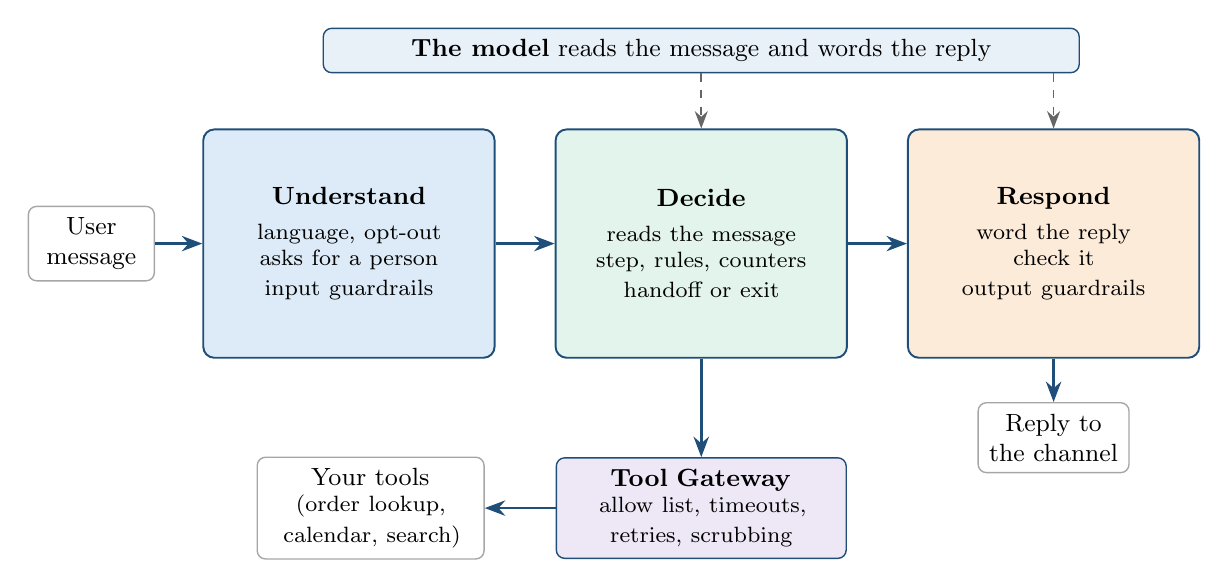
\begin{tikzpicture}[
  font=\small,
  stage/.style={draw=keel,fill=#1,rounded corners=4pt,minimum width=3.7cm,minimum height=2.9cm,
                align=center,text width=3.4cm,line width=0.7pt},
  ext/.style={draw=gray!70,fill=white,rounded corners=3pt,align=center,inner sep=4pt,line width=0.5pt},
  arr/.style={-{Stealth[length=2.6mm]},line width=0.9pt,color=keel},
  darr/.style={-{Stealth[length=2.2mm]},line width=0.6pt,color=gray!80!black,dashed},
  node distance=0.75cm]
  \node[ext,minimum width=1.6cm] (msg) {User\\message};
  \node[stage=boxA,right=0.6cm of msg] (u) {\textbf{Understand}\\[3pt]\footnotesize language, opt-out\\asks for a person\\input guardrails};
  \node[stage=boxB,right=of u] (d) {\textbf{Decide}\\[3pt]\footnotesize reads the message\\step, rules, counters\\handoff or exit};
  \node[stage=boxC,right=of d] (r) {\textbf{Respond}\\[3pt]\footnotesize word the reply\\check it\\output guardrails};
  \node[ext,below=0.55cm of r,minimum width=1.6cm] (rep) {Reply to\\the channel};
  \draw[arr] (msg) -- (u);
  \draw[arr] (u) -- (d);
  \draw[arr] (d) -- (r);
  \draw[arr] (r) -- (rep);
  % gateway
  \node[ext,below=1.25cm of d,fill=boxD,draw=keel,text width=3.4cm] (gw)
     {\textbf{Tool Gateway}\\\footnotesize allow list, timeouts,\\retries, scrubbing};
  \node[ext,left=0.9cm of gw,text width=2.6cm] (tools) {Your tools\\\footnotesize(order lookup,\\calendar, search)};
  \draw[arr] (d) -- (gw);
  \draw[arr] (gw) -- (tools);
  % model
  \node[ext,above=0.7cm of d,fill=keellight,draw=keel,minimum width=9.6cm] (llm)
     {\textbf{The model} reads the message and words the reply};
  \draw[darr] (llm.south -| d) -- (d.north);
  \draw[darr] (llm.south -| r) -- (r.north);
  \node[font=\scriptsize\itshape,color=gray!70!black,below=0.05cm of d.south,anchor=north west,xshift=0.08cm] {};
\end{tikzpicture}
\caption{Understand $\rightarrow$ Decide $\rightarrow$ Respond. Tools are reached only through the Tool Gateway.}
\end{figure}

\begin{description}[leftmargin=0pt,style=nextline]
  \item[Understand] keelchat detects the language, runs the input guardrails (for example
    \code{prompt\_injection}, which blocks attempts to trick the bot).
  \item[Decide] The model reads the message: a new answer, a change to an earlier answer, a side question, or
    something off-topic. Code turns that into counts and decisions. The current step of your \key{flow} runs. Answers are checked against what you said to
    \key{expect}. Re-asks, side trips and failures are counted against your \key{limits}. Rules that fit are
    added. If a tool is needed, it is called through the \textbf{Tool Gateway}, which only allows tools the
    policy lists, applies timeouts and retries, and treats tool output as data, never as instructions.
  \item[Respond] The model words the reply in the charter's tone. A checker makes sure nothing was invented, the
    output guardrails run (\code{pii} always removes personal details that should not be shown), and the
    channel shapes the message (for example SMS splits it into 160-character pieces).
\end{description}

\subsection{The deployment picture}

``Deployment'' means where the pieces run. In the simplest setup it is all \emph{one} server process; the
extra services are optional and only needed when you grow.

\begin{figure}[h]
\centering
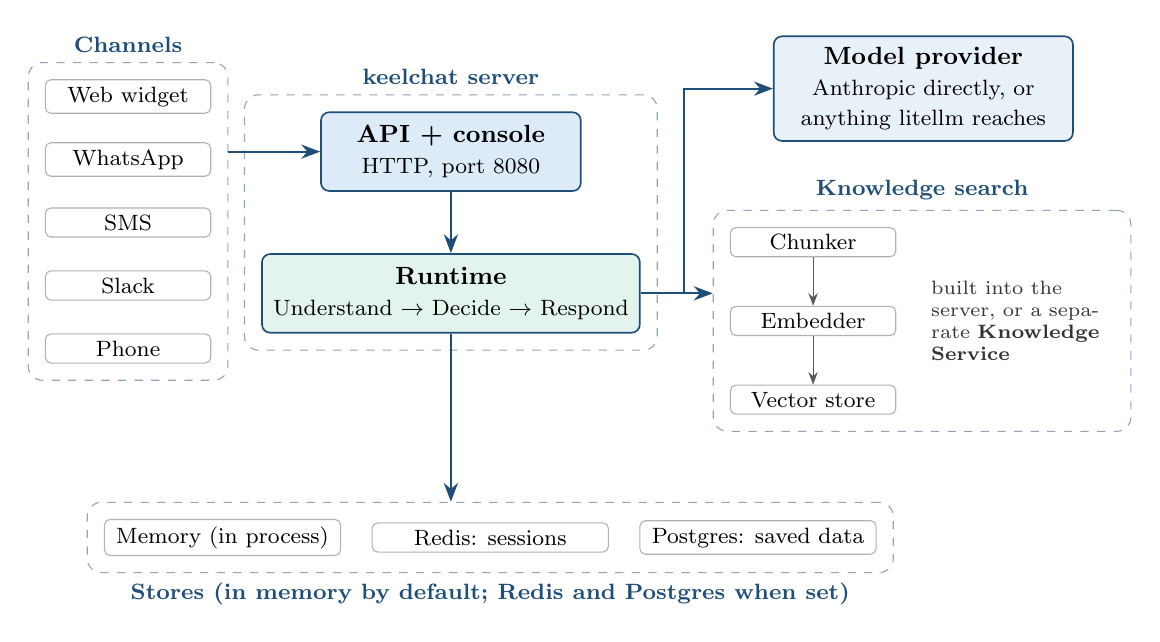
\begin{tikzpicture}[
  font=\small,
  box/.style={draw=keel,fill=#1,rounded corners=3pt,align=center,inner sep=4pt,line width=0.6pt},
  sm/.style={draw=gray!60,fill=white,rounded corners=2pt,align=center,inner sep=2.5pt,font=\footnotesize,minimum width=2.1cm},
  arr/.style={-{Stealth[length=2.4mm]},line width=0.8pt,color=keel},
  grp/.style={draw=keel!50,dashed,rounded corners=5pt,inner sep=6pt}]
  % channels
  \node[sm] (c1) at (0,3.0) {Web widget};
  \node[sm] (c2) at (0,2.2) {WhatsApp};
  \node[sm] (c3) at (0,1.4) {SMS};
  \node[sm] (c4) at (0,0.6) {Slack};
  \node[sm] (c5) at (0,-0.2) {Phone};
  \node[grp,fit=(c1)(c5),label={[font=\footnotesize\bfseries,color=keel]above:Channels}] (chg) {};
  % api
  \node[box=boxA,minimum width=3.3cm,minimum height=1.0cm] (api) at (4.1,2.3) {\textbf{API + console}\\\footnotesize HTTP, port 8080};
  \node[box=boxB,minimum width=3.3cm,minimum height=1.0cm] (rt) at (4.1,0.5) {\textbf{Runtime}\\\footnotesize Understand $\rightarrow$ Decide $\rightarrow$ Respond};
  \node[grp,fit=(api)(rt),label={[font=\footnotesize\bfseries,color=keel]above:keelchat server}] (srv) {};
  \draw[arr] (chg.east |- api) -- (api.west);
  \draw[arr] (api) -- (rt);
  % model provider
  \node[box=keellight,minimum width=3.8cm] (llm) at (10.1,3.1) {\textbf{Model provider}\\\footnotesize Anthropic directly, or\\\footnotesize anything litellm reaches};
  % knowledge
  \node[sm] (k1) at (8.7,1.15) {Chunker};
  \node[sm] (k2) at (8.7,0.15) {Embedder};
  \node[sm] (k3) at (8.7,-0.85) {Vector store};
  \draw[-{Stealth[length=1.6mm]},gray!70!black] (k1) -- (k2);
  \draw[-{Stealth[length=1.6mm]},gray!70!black] (k2) -- (k3);
  \node[align=left,font=\scriptsize,color=gray!40!black,text width=2.2cm] (kn) at (11.3,0.15)
    {\raggedright built into the server, or a separate \textbf{Knowledge Service}};
  \node[grp,fit=(k1)(k3)(kn),label={[font=\footnotesize\bfseries,color=keel]above:Knowledge search}] (kg) {};
  % stores
  \node[sm,minimum width=3.0cm] (s1) at (1.2,-2.6) {Memory (in process)};
  \node[sm,minimum width=3.0cm] (s2) at (4.6,-2.6) {Redis: sessions};
  \node[sm,minimum width=3.0cm] (s3) at (8.0,-2.6) {Postgres: saved data};
  \node[grp,fit=(s1)(s3),label={[font=\footnotesize\bfseries,color=keel]below:Stores (in memory by default; Redis and Postgres when set)}] (sg) {};
  \coordinate (fork) at ($(rt.east)+(0.55,0)$);
  \draw[line width=0.8pt,color=keel] (rt.east) -- (fork);
  \draw[arr] (fork) |- (llm.west);
  \draw[arr] (fork) -- (kg.west |- fork);
  \draw[arr] (rt.south) -- (sg.north -| rt.south);
\end{tikzpicture}
\caption{Channels talk to the API; the runtime calls the model provider, knowledge search and the stores.}
\end{figure}

\begin{itemize}[leftmargin=1.2em]
  \item \textbf{Channels} turn each platform's messages into one common form, and each channel owns its own
    limits and rules (for example SMS answers \code{STOP} before the bot sees it).
  \item \textbf{API + console}: one process serves both the HTTP API and the console web app.
  \item \textbf{Model provider}: keelchat calls Anthropic directly, or any provider that
    \emph{litellm} (a library that speaks to many AI providers) reaches: OpenAI, Gemini, Bedrock,
    OpenRouter, Ollama and more.
  \item \textbf{Knowledge search}: documents are split into passages (\emph{chunker}), turned into lists of
    numbers that capture meaning (\emph{embedder}), and kept where they can be searched by meaning
    (\emph{vector store}). The server does this itself; for large sets you run the separate Knowledge Service.
  \item \textbf{Stores}: where state is kept. With nothing set, everything is in memory and is lost when the server
    stops. Redis keeps sessions; Postgres keeps memory, saved bot versions, datasets, the audit log and handoffs.
\end{itemize}

% =================================================================
\section{Getting set up}
% =================================================================

Pick one of these paths. You can start with the first and move on later.

\begin{center}
\begin{tabularx}{\textwidth}{@{}L{4.0cm}L{2.0cm}Y@{}}
\toprule
\textbf{Path} & \textbf{Time} & \textbf{You need} \\
\midrule
Try it in your browser & 1 minute & Nothing \\
Run it on your computer & 5 minutes & macOS, Linux or WSL 2 (Linux inside Windows), and a model key \\
Install the Python package & 5 minutes & Python 3.12 or newer, and a model key \\
Deploy to Render & 10 minutes & GitHub and Render accounts, and a model key \\
\bottomrule
\end{tabularx}
\end{center}

\subsection{In the browser}

Open \url{https://keelchat-demo.fly.dev}. No sign-in is needed. Describe a bot, click through a few questions
about what your description leaves open (emergencies, what to collect, languages), and you get its YAML. Press
\textbf{Try this bot} to chat with it; its tools answer with sample data. A link can even start a draft:

\begin{lstlisting}[style=bashstyle]
https://keelchat-demo.fly.dev/?describe=Book+haircuts+and+ask+for+a+phone+number
\end{lstlisting}

\subsection{On your computer}

\begin{lstlisting}[style=bashstyle]
git clone https://github.com/pnrajan/keelchat && cd keelchat
./setup.sh        # checks for git, curl, uv, Node 20+; offers to install what's missing;
                  # asks for your model key and writes it to .env
scripts/try.sh    # opens the console with a sample bot, everything in memory
\end{lstlisting}

\code{uv} is a fast tool that installs Python and the project's libraries for you, so you don't need to manage a
``virtual environment'' by hand. \code{scripts/try.sh} opens \url{http://127.0.0.1:8000/console/}; in the
console, open \textbf{Compose}, describe a bot, press \textbf{Create my bot}, then \textbf{Try it}.

Other ways to run it locally:
\begin{itemize}[leftmargin=1.2em]
  \item \code{./run.sh} starts the console, the API and the Knowledge and Analytics Services, with sample
    documents and sample data. Use it for the document and data recipes.
  \item \code{scripts/local.sh up} runs the whole stack in Docker (API, console, Redis, Postgres), and keeps your
    data between restarts.
\end{itemize}

\subsection{As a Python package}

keelchat is on PyPI, the public index of Python packages. The \code{[api]} part is an \emph{extra}: it also
installs what the web server needs.

\begin{lstlisting}[style=bashstyle]
pip install "keelchat[api]"      # needs Python 3.12 or newer
keelchat build my_bot.yaml       # check a policy
keelchat serve --port 8000       # run the API
\end{lstlisting}

In a checkout of the repository you put \code{uv run} in front of each command
(\code{uv run keelchat build my\_bot.yaml}); with \code{pip install} the command is simply \code{keelchat}.

\subsection{The model key, in \texttt{.env}}

keelchat reads its settings from environment variables. It loads them from a file named
\code{.env}, which \code{./setup.sh} writes for you; \code{.env.example} lists the options. The minimum is a provider and its key:

\begin{lstlisting}[style=bashstyle]
# Anthropic directly
KEELCHAT_LLM=anthropic
ANTHROPIC_API_KEY=sk-ant-...

# or anything litellm reaches (also set the two model tiers and that provider's key)
# KEELCHAT_LLM=litellm
# KEELCHAT_MODEL_GENERATE=...    # writes replies
# KEELCHAT_MODEL_CLASSIFY=...    # reads messages, checks answers
# OPENROUTER_API_KEY=...
\end{lstlisting}

\begin{warn}[There is no pretend model]
keelchat always calls a real model, even in tests. A missing key stops it with an error instead of quietly
using a fake. That way, what passes in testing is what runs for real.
\end{warn}

\subsection{Deploy to Render}

Render is a hosting service with a free plan.
\begin{enumerate}[leftmargin=1.4em]
  \item \textbf{Fork} the keelchat repository on GitHub (make your own copy), so the deploy follows your copy.
  \item Open \code{https://render.com/deploy?repo=https://github.com/<you>/keelchat}.
  \item Sign in, review the service, enter your \code{ANTHROPIC\_API\_KEY} when asked, and approve. The first build
    takes a few minutes.
  \item On the service's \textbf{Environment} page, copy \code{KEELCHAT\_API\_KEY}. Render generated it; it locks
    the console and the API.
  \item Open \code{https://<service>.onrender.com}. The console asks for the key once.
\end{enumerate}

\begin{warn}[Saved bots need a database]
Without \code{DATABASE\_URL} (and \code{REDIS\_URL}), everything is in memory and is lost when the service restarts
or sleeps. Add a Postgres URL on the \textbf{Environment} page. The free plan also sleeps when idle, so the first
request after a quiet spell is slow.
\end{warn}

% =================================================================
\section{Your first bot}
% =================================================================

\subsection{The two-line bot}

The smallest bot has just two keys. Everything else has a sensible default.

\snip{01_first_bot.yaml}

\begin{itemize}[leftmargin=1.2em]
  \item \key{agent} is the bot's id: lowercase letters, digits and dashes.
  \item \key{charter} says what it helps with. Good charters also say the tone and what is out of scope.
\end{itemize}

With no \key{flow}, this bot simply chats within its charter. The default guardrails still run: prompt injection
is blocked and personal details are removed from replies.

\subsection{Build it}

``Building'' checks the file and compiles it into the form the runtime uses. Save the two lines as
\code{my\_bot.yaml} and run:

\begin{lstlisting}[style=bashstyle]
uv run keelchat build my_bot.yaml
\end{lstlisting}

If the file is fine, it prints the compiled policy. If not, every error names the exact place in the YAML. For
example, a rule with \code{handoff: true} but no top-level \key{handoff} key gives:

\begin{lstlisting}[style=bashstyle]
policy invalid:
  rules[0].handoff: a rule that hands off needs a top-level `handoff:`
    (e.g. `handoff: {when: [user_request]}`)
\end{lstlisting}

\code{rules[0]} means ``the first rule'' (counting starts at 0).

\subsection{Try it in the console}

\begin{enumerate}[leftmargin=1.4em]
  \item Start the console (\code{scripts/try.sh}).
  \item Open \textbf{Editor · test chat}, paste the YAML and press \textbf{Build \& try}. The editor completes keys,
    shows docs when you hover, and marks errors on their line as you type.
  \item Chat with the bot in the pane beside it. The \textbf{Inspector} on the right shows \emph{why} each reply
    was chosen: the step, the rule that fired, and how the reply was planned.
  \item Happy with it? Press \textbf{Save version}. Only valid builds can be saved, and each one gets a number so
    you can compare and roll back.
\end{enumerate}

Or skip the YAML: in \textbf{Compose}, say what the bot should do in a sentence, read what it will do in plain
words, and ask for changes the same way (``also ask for their email'').

\subsection{Try it through the API}

The console uses an HTTP API, and so can your own programs. Three calls make a conversation. Here they are with
\code{curl} (a command-line tool that sends web requests) and \code{jq} (a tool that reads JSON):

\begin{lstlisting}[style=bashstyle]
API=http://127.0.0.1:8000

# 1. Build the policy (errors come back as YAML paths, like keelchat build)
curl -s $API/v1/agents -H 'content-type: application/json' \
  -d "$(jq -n --rawfile y my_bot.yaml '{yaml: $y}')"

# 2. Open a session (one conversation) with that bot
SID=$(curl -s $API/v1/sessions -H 'content-type: application/json' \
  -d '{"agent": "shop-helper", "user_id": "dev"}' | jq -r .id)

# 3. Send a message and read the reply
curl -s $API/v1/sessions/$SID/turns -H 'content-type: application/json' \
  -d '{"text": "Hi, where is my order?"}' | jq .outbound.text
\end{lstlisting}

\begin{note}
If the server has \code{KEELCHAT\_API\_KEY} set, add \code{-H "Authorization: Bearer \$KEELCHAT\_API\_KEY"} to
each call. Interactive API docs are at \code{/docs} on the server. A \emph{session} stays on the policy version
it started with, so changing a bot never changes a chat that is already going.
\end{note}

% =================================================================
\section{Recipes: one per kind of bot}
% =================================================================

Each recipe gives the YAML (built and checked), explains each part, and says how to try it.

% -----------------------------------------------------------------
\subsection{Support assistant: collect an order number, then hand over}
\recipehead{order problems, returns, account questions.}{\key{form\_fill} step, a rule, guardrails, limits, \key{handoff}.}

\snip{02_support.yaml}

\textbf{What each part does}
\begin{itemize}[leftmargin=1.2em]
  \item \key{greet\_consent} greets the person and asks if it may use and remember their answers.
  \item \key{form\_fill} asks one field at a time. \key{ask} is a \emph{sample} question: the model words it to fit
    the conversation. \key{expect} is what counts as a valid answer, written as you would explain it to a person,
    not as a pattern. Answers that don't fit are asked again. \key{closing} is said once every field is answered.
  \item The \key{damaged\_item} rule adds its \key{then} to the reply only on a message that fits its \key{when}.
  \item \key{guardrails}: \code{prompt\_injection} and \code{pii} always run; \code{no\_legal\_advice} is added because the
    charter rules out legal advice.
  \item \key{limits}: at most 3 re-asks of one question, and 3 off-topic turns in a row before it steers back.
  \item \key{handoff}: the chat goes to a person when they ask (\code{user\_request}) or when an answer fails too
    often (\code{max\_reasks}).
\end{itemize}

\textbf{How to try it.} Build \& try, then: ``hi'', ``yes'', ``my shoes arrived broken'' (the rule should fire, and
the Inspector shows it), ``ORD-12345'', then ``the sole came off''. Start again and type ``can I talk to a human?''
to see the handoff. Handed-over chats appear in the console's \textbf{Handoffs} tab.

\begin{tip}[Make the bot more careful]
The repository's \code{examples/support\_assistant.yaml} adds \code{think: true} (plan each reply first) and
\code{curious: true} (one follow-up when an answer is too thin, such as ``it's broken''). Both cost an extra model
call, so they are off by default. See Section~\ref{sec:behave}.
\end{tip}

% -----------------------------------------------------------------
\subsection{Appointment booking with an emergency rule}
\recipehead{clinics, salons, any ``book a slot'' service where some messages must go to a person at once.}%
{\key{form\_fill}, a rule with \code{handoff: true}, a top-level \key{handoff}.}

\snip{03_booking.yaml}

\textbf{What each part does}
\begin{itemize}[leftmargin=1.2em]
  \item The four fields collect what the front desk needs. \key{languages} lists English and Spanish; the bot
    detects the language, confirms before switching, and answers in it.
  \item The \key{dental\_emergency} rule has \code{handoff: true}. When it matches, the conversation passes to a
    person \emph{in code}: the reply says so and asks nothing more. The handoff's reason is
    \code{rule:dental\_emergency}.
  \item \code{handoff: true} on a rule \textbf{needs} the top-level \key{handoff} key, or the build fails (you saw
    that error in Section 4).
  \item \code{no\_medical\_advice} matches the charter's ``Out of scope: medical advice''.
\end{itemize}

\textbf{Why this matters.} When the emergency instruction only lives in a prompt, a bot might say ``I need to
connect you with a staff member'' and then carry on asking which treatment you want, with nobody getting the
chat. With the rule in code, a person gets it every time.

\textbf{How to try it.} Start booking, then write ``I just knocked a tooth out playing football''. The reply should
say a person is taking over, and the chat should appear in \textbf{Handoffs}.

\begin{note}[Booking real slots]
This bot collects a preferred day; the front desk confirms the time. To offer real free slots, you add a tool and
a step of your own. The repository's \code{examples/booking\_assistant.yaml} does this with an extension package
(a \code{slot\_search} tool and a \code{pick\_slot} step). Recipe~\ref{sec:tool} shows how to write a tool.
\end{note}

% -----------------------------------------------------------------
\subsection{Customer survey (NPS)}
\recipehead{after-purchase feedback, satisfaction scores, short questionnaires.}%
{\key{survey} step with questions of different kinds; \code{ask\_if} for follow-ups.}

NPS (Net Promoter Score) is the classic ``How likely are you to recommend us, from 0 to 10?'' question.

\snip{04_survey.yaml}

\textbf{What each part does}
\begin{itemize}[leftmargin=1.2em]
  \item \key{survey} asks its \key{questions} in order and records each answer and how it was captured.
  \item The \key{key} \code{nps} makes the answer an NPS score. \code{kind: scale} with \key{scale\_min}/\key{scale\_max}
    and labels for the ends. Closed kinds (\code{scale}, \code{single\_choice}, \code{multi\_choice}, \code{rank},
    \code{allocation}, \code{number}) are read in code; a messy reply (``my sister told me'') is interpreted and
    read back for the person to confirm.
  \item Open questions (the default \key{kind}) are conversational: \key{expectation} says what a complete answer
    covers, and the bot asks up to \key{max\_probes} follow-ups until it does.
  \item \key{ask\_if} asks a question only when an earlier answer meets a condition, decided in code. Here, a score
    of 6 or less gets ``What could we have done better?'' and 7 or more gets ``What did you like most?''.
\end{itemize}

\textbf{Prefer a natural chat over fixed questions?} \key{conversation\_survey} takes \emph{objectives} (what you
want to learn) and finds each out in a natural conversation, skipping what the person already said:

\snip{04b_conversation_survey.yaml}

\textbf{How to try it and see results.} Answer it a few times with low and high scores. Finished surveys are kept
for findings: \code{GET /v1/tenants/\{t\}/agents/\{agent\}/findings} gives counts and NPS (computed in code) and
themes with real quotes; \code{.../responses.csv} downloads the answers. The console's \textbf{Publish · results}
shows scores over time. A shared link with \code{?score=8} starts the survey with a score already clicked, which
is handy in an email.

% -----------------------------------------------------------------
\subsection{Answering from your documents}
\recipehead{help centres, product manuals, FAQs, policies.}{a knowledge base and a \key{knowledge} step with \key{dataset}.}

A \textbf{knowledge base} is a named set of your documents. The bot answers \emph{only} from passages it finds
there, and each answer is checked against them. When the documents don't cover a question, the bot says so
instead of guessing.

\subsubsection{Step 1: make the knowledge base}

\textbf{In the console:} Compose $\rightarrow$ \textbf{Knowledge base}. Upload files (PDF, text, Markdown, CSV,
HTML) or add web pages, press \textbf{Create knowledge base}, then apply the change it proposes. Or use Publish
$\rightarrow$ \emph{Create a chatbot from your content} to make a whole bot from documents in one go.

\textbf{By API:} send files and web addresses as a form upload (\code{-F} sends one form field):

\begin{lstlisting}[style=bashstyle]
curl -s -X POST $API/v1/tenants/default/documents \
  -F agent=help-centre -F name=help_centre \
  -F files=@returns-policy.pdf -F files=@delivery.md \
  -F urls=https://example.com/help/warranty
# -> {"dataset": "help_centre", "documents": [...], ...}
#    plus the indexing method it picked, and why
\end{lstlisting}

A \emph{tenant} is one customer account on a keelchat server; on your own server it is \code{default}.
\code{name} names the knowledge base (default \code{kb\_<agent>}). Documents already in a folder or S3 can be
registered with \code{PUT /v1/tenants/\{t\}/datasets/\{name\}}.

\subsubsection{Step 2: the bot}

\snip{05_knowledge.yaml}

The \key{knowledge} step's \key{dataset} names the knowledge base. Several bots can share one.

\textbf{Side questions in another bot.} A bot with a form can also answer side questions from documents: list the
\code{knowledge\_search} tool under \key{tools}. The question is answered and the open question is asked again.

\snip{05b_knowledge_shared.yaml}

\textbf{How it's indexed.} ``Indexing'' prepares the documents for search. With the default (\code{auto}), keelchat
picks the method and tells you why:

\begin{center}
\small
\begin{tabularx}{\textwidth}{@{}L{4.4cm}L{2.6cm}Y@{}}
\toprule
\textbf{Documents} & \textbf{Method} & \textbf{What it does} \\
\midrule
Fit in one prompt (about 40,000 characters) & \code{full\_context} & The bot reads every document whole \\
Long documents (a manual) & \code{raptor} & Summaries at several levels, for broad and detailed questions \\
Many shorter documents & \code{contextual} & Each passage gets a line of context so search finds the right one \\
No model to index with & \code{simple} & Passages found by meaning \\
\bottomrule
\end{tabularx}
\end{center}

\textbf{How to try it.} \code{./run.sh} starts the Knowledge Service with sample documents; otherwise the server
indexes knowledge bases itself. Ask something the documents answer, then something they don't: the bot should say
it doesn't know.

\begin{warn}
\code{keelchat build} on your own computer checks the YAML's shape. Whether the dataset \emph{exists} is checked
when you build on the server, where the knowledge base lives. Make the knowledge base first.
\end{warn}

% -----------------------------------------------------------------
\subsection{Data questions over a table}
\recipehead{``Which region sold most?'' over your own sales or operations data.}{a structured dataset and an \key{analytics} step.}

\snip{06_analytics.yaml}

A \textbf{structured dataset} is one or more tables (CSV or Parquet files). Questions become SQL (the language for
asking tables questions) run on a locked, in-memory copy of the data. Every answer is planned, checked and verified
before it is shown; numbers must come from the result. An answer that fails its checks is marked \emph{partial}.
\key{limits.repairs} is how many times a step may fix its own failed attempt (for example rewrite failing SQL).

\textbf{Register the dataset first.} Sources must sit under \code{KEELCHAT\_DATA\_ROOT}:

\begin{lstlisting}[style=bashstyle]
curl -s -X PUT $API/v1/tenants/default/datasets/sales \
  -H 'content-type: application/json' -d '{
  "description": "Online store orders, January to June 2026",
  "spec": {"kind": "structured", "tables": [
    {"name": "orders", "uri": "'"$PWD"'/examples/data/orders.csv",
     "columns": {"amount": "order total in USD"}},
    {"name": "targets", "uri": "'"$PWD"'/examples/data/targets.parquet",
     "description": "Quarterly revenue target per region"}]}}'
\end{lstlisting}

\textbf{How to try it.} \code{./run.sh} (or \code{scripts/dev.sh --analytics}) starts the Analytics Service and
registers the sample data as \code{sales} for you. Ask ``Which region brought in the most revenue?'' and then a
follow-up like ``and in March?''. Statistics code (beyond SQL) runs only in a sandbox with no network; turn it on
with \code{./run.sh --sandbox}.

% -----------------------------------------------------------------
\subsection{A bot that calls your own tool}\label{sec:tool}
\recipehead{looking things up in your own systems: order status, stock, opening hours.}%
{a Python function with \code{@tool}, listed in \key{tools}.}

A \textbf{tool} is an \code{async} Python function (one that can wait for a network reply without blocking).
keelchat turns its type hints into the input schema, and the \emph{docstring} (the text in triple quotes) is what
the model reads to decide when to use it.

\lstinputlisting[style=pystyle]{snippets/my_tools/orders.py}

\begin{itemize}[leftmargin=1.2em]
  \item \code{timeout\_s=3.0}: the gateway stops waiting after 3 seconds. \code{retries=1}: it tries once more after
    a timeout or error; after repeated failures a circuit breaker stops calling the tool for a while.
  \item Raise \code{ToolError(name, kind, message)} for failures. A dictionary stands in for your real system here.
  \item Tools only \emph{read}. Anything that changes something (book, pay, submit) must be an
    \code{@action} instead, which runs only on the user's own explicit action.
\end{itemize}

Now allow it in a policy:

\snip{07_tool.yaml}

\code{mode: planner} means there is no fixed list of steps: each turn the \emph{planner} picks read-only tools from the
allow list and answers from what they return. \key{limits.planner\_calls} caps tool calls per turn, counted in code.
\code{tool\_unavailable} in \key{handoff} passes the chat to a person if the tool is down.

\textbf{Make keelchat find your code.} Put the file in a package folder (here \code{my\_tools/} with an empty
\code{\_\_init\_\_.py}) and name the package in \code{KEELCHAT\_CAPABILITY\_PACKAGES}:

\begin{lstlisting}[style=bashstyle]
PYTHONPATH=. KEELCHAT_CAPABILITY_PACKAGES=my_tools \
  uv run keelchat build order_tracker.yaml
\end{lstlisting}

Without it the build stops with \code{tools[0]: unregistered tool 'order\_status'} and lists the tools it knows.

\begin{tip}[Start from a template]
\code{uv run keelchat new package acme\_caps --out my\_bot} writes a starter package with a tool, a step, a
guardrail, an agent that uses them, and a passing test. It is the quickest way to see how the parts fit.
\end{tip}

% =================================================================
\section{Making bots behave}\label{sec:behave}
% =================================================================

Here is a policy that uses most of the ``behaviour'' settings at once. Each one is explained below.

\snip{08_behave.yaml}

{\small
\begin{xltabular}{\textwidth}{@{}L{3.4cm}Y@{}}
\toprule
\textbf{Setting} & \textbf{What it does} \\
\midrule
\endhead
\key{rules} (\code{when}/\code{then}) & Applies only to messages that fit \code{when}. Write \code{when} about the
  customer's message (``asks for a refund over \$500''), not the mood of the chat. A match must quote the latest
  message, so an earlier message never fires a rule again. \code{overrides} settles conflicts between rules. \\
\key{limits} & Counted in code: \code{reasks} (per question, default 3), \code{digressions} (off-topic turns in a
  row, 3), \code{reopens} (edits to a finished step, 2), \code{planner\_calls} (6), \code{on\_step\_enquiries} (3),
  \code{repairs} (2). SMS users tolerate fewer re-asks than web users. \\
\key{guardrails} & Input: \code{prompt\_injection}, \code{sql\_injection}. Output: \code{pii}, \code{profanity},
  \code{no\_legal\_advice}, \code{no\_medical\_advice}. \code{prompt\_injection} and \code{pii} always run. \\
\key{memory} & Only the items you list are remembered between conversations, each typed and fading by
  \code{half\_life}. \code{sensitive: true} items need consent, must be volunteered, and never reach a tool.
  \code{confirm\_on\_reuse} asks ``is it still \ldots?''. Put \code{greet\_consent} first: without consent, sensitive items are never kept. \\
\key{languages} & Languages it speaks; the first is the fallback. List only ones you support end to end. \\
\key{small\_talk} & \code{off} (default: chit-chat counts as off-topic), \code{brief} (one friendly line, then back),
  \code{warm} (one or two sentences). Never taken as an answer. \\
\code{think: true} & On a step: plan each reply first (what they need, what is unknown, which rules apply). The plan
  shows in the Inspector's \textbf{Why} tab. One more model call. \\
\code{curious: true} & On a \code{form\_fill}: one follow-up when an answer is valid but too thin (``it's broken'' --
  broken how?). Never for ids, numbers, names, dates or yes/no. \\
\code{model: small|large} & On a step: run all its work on one model size. Simple steps can use \code{small} to
  save money. \\
\code{high\_stakes: true} & On a step or a rule: that turn's reply is written with the large model and always
  checked before sending. \\
\key{handoff} & \code{when}: \code{user\_request}, \code{max\_reasks}, \code{disengaged}, \code{tool\_unavailable}.
  \code{notify: handoff\_webhook} also sends it to your help desk (\code{HANDOFF\_URL}). \code{timeout} gives the chat
  back to the bot if nobody replies in time. \\
\key{mode} & \code{flow} (every reply from a step), \code{adaptive} (a multi-part side question may use the
  planner), \code{planner} (no fixed steps). \\
\bottomrule
\end{xltabular}}

\begin{tip}[Charter vs.\ settings]
Put scope and tone in the charter. Don't put limits or guardrails in the charter text: they belong in their own
keys, where code enforces them. Name the out-of-scope topics users actually bring up.
\end{tip}

\textbf{Durations} are a number and a unit: \code{s}, \code{m}, \code{h}, \code{d} or \code{w} (\code{90d},
\code{24h}). Text YAML would read as true/false (\code{yes}, \code{no}, \code{on}, \code{off}) needs quotes:
\code{"yes"}.

\subsection*{What happens on a handoff}
\begin{enumerate}[leftmargin=1.4em]
  \item \textbf{Triggered}: the user asks for a person, a rule with \code{handoff: true} matches, or a dead end in
    \code{when} is reached.
  \item \textbf{Sent}: a ticket opens in the handoff inbox (console \textbf{Handoffs} tab) with the reason, the answers
    so far and the recent transcript, with sensitive values removed.
  \item \textbf{Waiting}: later messages join the same ticket.
  \item \textbf{Reported back}: a person presses \textbf{Resolve and resume} or \textbf{Resolve and end}, or your help
    desk calls the ticket's \code{callback\_url}.
  \item \textbf{Resumed}: the bot says it is back and carries on from the next open question.
\end{enumerate}

% =================================================================
\section{Testing your bot}
% =================================================================

Test before real people use the bot. keelchat gives you three levels.

\subsection{In the console}

\begin{center}
\small
\begin{tabularx}{\textwidth}{@{}L{3.0cm}Y@{}}
\toprule
\textbf{Where} & \textbf{What you do} \\
\midrule
\textbf{Test $\rightarrow$ Tests} & Save a chat as a test, draft tests from the policy, run them all on the current
  build. \code{scripts/try.sh} saves three sample tests: press \textbf{Run}. \\
\textbf{Simulate} & Model-played personas (pretend customers) and scripted replays, on fake tools. \\
\textbf{Rate} & Mark each reply in scope or not, each rule followed or not; let the model suggest policy changes. \\
\textbf{Judge} & A stronger model (\code{KEELCHAT\_MODEL\_CRITIC}) reads a trial chat, lists what went wrong on which
  turn, and proposes fixes. Tick the policy fixes and \textbf{Apply to the policy}; the build checks them and nothing
  is saved until you save. \\
\bottomrule
\end{tabularx}
\end{center}

\subsection{From the command line}

An \emph{eval set} is a folder of test conversations for one bot, kept in \code{evals/<agent>/}.

\begin{lstlisting}[style=bashstyle]
uv run keelchat evals generate my_bot.yaml          # draft a test set
uv run keelchat evals run evals/support_assistant    # run it: checks done in code
uv run keelchat evals check evals/support_assistant  # also the judged checks
uv run keelchat simulate examples/hiring_agent.yaml examples/sim_script.yaml
\end{lstlisting}

A test case is plain YAML in \code{replay.yaml}: messages to send, and what must be true afterwards.

\begin{lstlisting}[style=yamlstyle]
cases:
  - name: happy_path
    messages: ["hi", "yes", "ORD-12345", "it never arrived"]
    expect: {completed: true, fields: {order_number: ORD-12345}}
  - name: damaged_item_rule
    messages: ["hi", "yes", "my blender arrived broken", "ORD-12345"]
    expect: {rules: {3: [damaged_item], 4: []}}   # turn 3 must match the rule
  - name: wants_a_person
    persona: Agrees to share answers, then insists on talking to a real person.
    max_turns: 6
    expect: {exit_reason: handed_off}
\end{lstlisting}

\begin{tip}[What to cover]
The happy path, every exit (too many re-asks, a person asked for), one edit (``actually my order number is
\ldots''), one message with two intents, one off-topic message, one per language, and one per rule. The judged
evals need \code{pip install "keelchat[evals]"} and a judge model (\code{EVALS\_JUDGE\_MODEL}).
\end{tip}

% =================================================================
\section{Extending keelchat with your own code}
% =================================================================

Every extension is \textbf{one decorated Python function or class}, registered by name. You never change the
runtime. Everything imports from the top level: \code{from keelchat import tool, node, guardrail, \ldots}.

\begin{center}
\small
\begin{tabularx}{\textwidth}{@{}L{2.7cm}L{5.0cm}Y@{}}
\toprule
\textbf{You add} & \textbf{How} & \textbf{Used in the policy as} \\
\midrule
Tool & \code{@tool("name")} & \code{tools: [name]} \\
Step & \code{@node("name")} on a \code{Node} class & a \key{flow} entry: \code{- name: \{...\}} \\
Guardrail & \code{@guardrail("name", stage="output")} & \code{guardrails: \{output: [pii, name]\}} \\
Action (commits) & \code{@action("name", by="candidate")} & runs only on the user's explicit action \\
MCP server tools & list in \code{KEELCHAT\_MCP\_SERVERS} & \code{tools: [alias.tool]} \\
HTTP endpoint & \code{POST /v1/tenants/\{t\}/tools} & \code{tools: [name]} \\
\bottomrule
\end{tabularx}
\end{center}

MCP (Model Context Protocol) is a standard way for programs to offer tools to AI models; any MCP server's tools
can be used without writing code. keelchat finds your package through the setting
\code{KEELCHAT\_CAPABILITY\_PACKAGES}, or through an entry point in your \code{pyproject.toml}. \code{check\_capability} runs the \emph{contract suite} (the checks every
capability must pass) on one of yours.

\subsection{Replacing parts of knowledge search}

Knowledge search has four parts you can swap. Each has an interface (a base class), a decorator that registers
your version by name, and a setting that picks it.

\begin{center}
\small
\begin{tabularx}{\textwidth}{@{}L{2.8cm}L{3.9cm}L{3.5cm}Y@{}}
\toprule
\textbf{Part} & \textbf{Interface} & \textbf{Register / setting} & \textbf{Built in} \\
\midrule
Embedding model & \code{Embedder}: \code{dim}, \code{id}, \code{embed(texts)} & \code{@embedder} /
  \code{KNOWLEDGE\_EMBEDDER} & litellm, chonkie, sentence-transformers, siliconflow, hash \\
Splitting into passages & \code{Chunker}: \code{chunk(text)} & \code{@chunker} / \code{KNOWLEDGE\_CHUNKER} & chonkie,
  semantic, sentences \\
Indexing method & \code{Indexer}: \code{chunks(doc)} & \code{@indexer} / \code{KNOWLEDGE\_STRATEGY} & simple,
  contextual, raptor, full\_context \\
Vector store & \code{VectorIndex}: \code{upsert}, \code{search}, \code{delete\_doc}, \code{count} &
  \code{@vector\_store} / \code{KNOWLEDGE\_VECTOR\_STORE} & memory, lancedb, qdrant, chroma, pgvector \\
\bottomrule
\end{tabularx}
\end{center}

Here is a complete, tiny vector store that keeps vectors in a Python dictionary, with its test. It was run, and
\code{check\_vector\_store} passed.

\lstinputlisting[style=pystyle,lastline=46]{snippets/vector_store_demo.py}

A vector store must keep datasets apart, honour \code{max\_level}, replace a chunk upserted again with the same id,
and return whole chunks with cosine similarity as the score. \code{check\_vector\_store} tests all of that on an
empty store and names the rule that failed. Then pick it with \code{KNOWLEDGE\_VECTOR\_STORE=dictstore}.

\begin{note}
A real store would talk to a database; this one forgets everything on restart, like the built-in
\code{memory} store. Switching embedders re-indexes the documents rather than mixing vectors that can't be
compared.
\end{note}

% =================================================================
\section{Going live}
% =================================================================

\subsection{Channels and Publish}

The console's \textbf{Channels} tab says what to paste or configure for each one.

\begin{center}
\small
\begin{tabularx}{\textwidth}{@{}L{3.2cm}Y@{}}
\toprule
\textbf{Channel} & \textbf{How it connects} \\
\midrule
Website widget & Publish the agent (\code{POST /v1/tenants/\{t\}/agents/\{agent\}/embeds}) and paste the one-line
  \code{<script>} it returns. Only the sites you list can show it. \\
Link and app & The same publish returns \code{app\_url}: a full-screen chat that installs on a phone. \\
WhatsApp & WhatsApp Cloud API: \code{POST .../embeds/\{id\}/whatsapp} stores the number's token encrypted. \\
Phone & Point a Twilio number's voice webhook at \code{/v1/public/phone/embeds/\{id\}}. \\
SMS & Post Twilio's form fields as the turn's \code{payload}; long replies are split, STOP is answered. \\
Slack & Post the Slack event as the turn's \code{payload}; lists become Slack blocks. \\
\bottomrule
\end{tabularx}
\end{center}

\subsection{API keys}

\code{KEELCHAT\_API\_KEY} is the admin key. Give each website or messaging backend its own key with
\code{POST /v1/tenants/\{t\}/keys}; each is shown once and stored as a hash, and reaches only its own tenant.

\begin{center}
\small
\begin{tabularx}{0.8\textwidth}{@{}L{2.4cm}Y@{}}
\toprule
\textbf{Scope} & \textbf{Allows} \\
\midrule
\code{build} & everything in its tenant \\
\code{read} & read-only access \\
\code{runtime} & sessions and turns only: the key for a website or messaging backend \\
\bottomrule
\end{tabularx}
\end{center}

\subsection{Checklist before real customers}

\begin{tcolorbox}[enhanced,colback=white,colframe=keel,arc=3pt,boxrule=0.6pt,left=8pt,right=8pt]
\small
\begin{itemize}[label={$\square$},leftmargin=1.4em,itemsep=0.25em]
  \item A database is set: \code{DATABASE\_URL} (Postgres) and \code{REDIS\_URL}, so saved bots and chats survive
    restarts (\code{scripts/db.sh up} starts both locally).
  \item \code{KEELCHAT\_API\_KEY} is set, and the website uses a \code{runtime}-scoped key, not the admin key.
  \item The charter names the out-of-scope topics users actually bring up.
  \item Every step asks one thing; every \code{expect} reads like an instruction to a person.
  \item Limits suit the channel; \key{handoff} is set, and someone watches the Handoffs inbox (or \code{notify}
    sends to your help desk).
  \item Memory items are typed, have a half-life, and sensitive ones are marked.
  \item Anything that commits (book, pay, submit) is an action, not a tool.
  \item Tools point at real systems (not \code{KEELCHAT\_TOOLS=fake}, which is for development only).
  \item \code{keelchat build} and \code{keelchat evals run} are green.
  \item Set \code{KEELCHAT\_PUBLIC\_URL} so links and help-desk callbacks have a full address.
\end{itemize}
\end{tcolorbox}

After launch, the \textbf{Outcomes} dashboard shows how conversations ended, and the audit log
(\code{GET /v1/tenants/\{t\}/audit}) records every decision. \code{keelchat evals export} turns a failed live
conversation into a test case.

\clearpage
% =================================================================
\section{Troubleshooting}
% =================================================================

\begin{center}
\small
\begin{tabularx}{\textwidth}{@{}L{5.6cm}Y@{}}
\toprule
\textbf{What you see} & \textbf{What to do} \\
\midrule
A reply says it can't do something ``right now'' (``I can't look that up right now\ldots'') & The tool's service is
  down or its URL is unset: start it (\code{./run.sh} starts Knowledge and Analytics), or run with
  \code{./run.sh --fake-tools} (or set \code{KEELCHAT\_TOOLS=fake}). \\
``The API no longer has this policy'' or ``This session is no longer on the server'' & The API restarted with
  in-memory state: \textbf{Build \& try} again and start a new session, or set \code{DATABASE\_URL} and
  \code{REDIS\_URL}. \\
The API exits at start with a database error & \code{DATABASE\_URL} names a database that doesn't exist:
  \code{scripts/db.sh up}, or leave it empty. \\
\textbf{Save version} is disabled & The editor found problems; only valid builds are saved. Fix the marked lines. \\
The console shows ``API offline'' & The API process is down: check the terminal running \code{./run.sh}. \\
\code{./setup.sh} stops on a missing tool & It lists what's missing and the command it would run: rerun with
  \code{--yes}, or install them yourself. On Windows, run it inside WSL 2. \\
\code{scripts/local.sh up} says Docker is not running & Start Docker Desktop (macOS, Windows) or
  \code{sudo systemctl start docker} (Linux). \\
\code{scripts/local.sh up}: the API container exits & Run \code{scripts/local.sh logs}; usually there is no model
  key in \code{.env}. \\
\code{keelchat build}: \code{unregistered tool} & Your package isn't loaded: set \code{PYTHONPATH} and
  \code{KEELCHAT\_CAPABILITY\_PACKAGES}. \\
\code{keelchat build}: \code{a rule that hands off needs a top-level `handoff:`} & Add
  \code{handoff: \{when: [user\_request]\}}. \\
\bottomrule
\end{tabularx}
\end{center}

Every log line carries a \code{session\_id}, so searching the logs for it follows one conversation from start to
end.

\begin{panel}{Where to read more}
\small
In the repository's \code{docs/} folder: \textbf{WRITING\_AN\_AGENT.md} (writing and tuning a bot),
\textbf{POLICY\_LANGUAGE.md} (every policy key, its values and defaults), \textbf{FEATURES.md} (console, channels,
memory, handoff, documents), \textbf{ADDING\_A\_CAPABILITY.md} (tools, steps, guardrails, channels, knowledge
search parts), \textbf{EVALS.md} (testing), \textbf{REFERENCE.md} (CLI, API, settings, deployment) and
\textbf{ARCHITECTURE.md} (how the runtime works). The \code{examples/} folder has bots for support, bookings,
surveys, hiring, a hotel concierge and data questions.
\end{panel}

\end{document}
